\documentclass[12pt,UTF8]{ctexart}
\usepackage{graphicx} % Required for inserting images
\usepackage{amsmath}
\usepackage{graphicx}
\usepackage{geometry}
\usepackage{fancyhdr}
\usepackage{pythonhighlight}
%\usepackage{setspace}
\usepackage{caption}
\usepackage{cite}
\usepackage{multicol}
\usepackage{enumitem}
\usepackage{titlesec}
\usepackage{matlab-prettifier}
\geometry{papersize={20cm,27cm}}
\geometry{left=2cm,right=2cm,top=2cm,bottom=2cm}
\title{Matlab Retard Elementary Homework NO.1}
\pagestyle{fancy}
\author{ChatGPT Conjurator Nellurkia}
\date{2024/3/30}


\lfoot{}
\cfoot{\thepage}
\rfoot{}
\renewcommand{\headrulewidth}{0.4pt}
\renewcommand{\headwidth}{\textwidth}
\renewcommand{\footrulewidth}{0pt}
\usepackage{setspace}
\onehalfspacing
\addtolength{\parskip}{.4em}
\newcommand{\subsubsubsection}[1]{\paragraph{#1}\mbox{}\\}
\setcounter{secnumdepth}{4} % how many sectioning levels to assign numbers to
\setcounter{tocdepth}{4} % how many sectioning levels to show in ToC
\usepackage{indentfirst}
\setlength{\parindent}{2em}

\begin{document}

\maketitle

\clearpage

\begin{figure}
    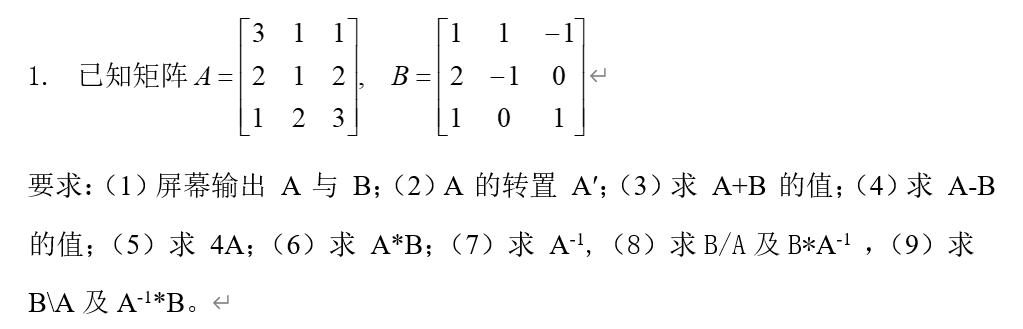
\includegraphics[width=1\linewidth]{image.png}
\end{figure}

\par \textbf{思路简介}
\par 根据题意由matlab矩阵语法即得。
\par \textbf{解答}

\begin{lstlisting}[
frame=single,
numbers=left,
style=Matlab-Pyglike]
A = [3 1 1; 2 1 2; 1 2 3]
B = [1 1 -1; 2 -1 0; 1 0 1]
A'
A+B
A-B
4*A
A*B
inv(A)
B/A
B*inv(A)
B\A
inv(A)*B
\end{lstlisting}

\par \textbf{实验结果}

\begin{lstlisting}[
frame=single,
numbers=left]
    >> hw1

A =

     3     1     1
     2     1     2
     1     2     3


B =

     1     1    -1
     2    -1     0
     1     0     1


ans =

     3     2     1
     1     1     2
     1     2     3


ans =

     4     2     0
     4     0     2
     2     2     4


ans =

     2     0     2
     0     2     2
     0     2     2


ans =

    12     4     4
     8     4     8
     4     8    12


ans =

     6     2    -2
     6     1     0
     8    -1     2


ans =

    0.2500    0.2500   -0.2500
    1.0000   -2.0000    1.0000
   -0.7500    1.2500   -0.2500


ans =

    2.0000   -3.0000    1.0000
   -0.5000    2.5000   -1.5000
   -0.5000    1.5000   -0.5000


ans =

    2.0000   -3.0000    1.0000
   -0.5000    2.5000   -1.5000
   -0.5000    1.5000   -0.5000


ans =

    1.5000    1.0000    1.5000
    1.0000    1.0000    1.0000
   -0.5000    1.0000    1.5000


ans =

    0.5000    0.0000   -0.5000
   -2.0000    3.0000    0.0000
    1.5000   -2.0000    0.5000

>> 
\end{lstlisting}

\clearpage
\begin{figure}
    \centering
    
\includegraphics[width=1\linewidth]{++2.png} 
\end{figure}

\par \textbf{思路简介}
\par 根据题意,通过调用函数来计算结果。
\par \textbf{解答}

\begin{lstlisting}[
frame=single,
numbers=left,
style=Matlab-Pyglike]
x = input('请输入 x 的值:');
y = input('请输入 y 的值:');

result = hw2_(x, y);

disp(['函数值为:', num2str(result)]);
\end{lstlisting}
\begin{lstlisting}[
frame=single,
numbers=left,
style=Matlab-Pyglike]
function result = hw2_(x, y)
    result = x^2 + sin(x*y) + 2*y;
end
\end{lstlisting}

\par \textbf{实验结果}

\begin{lstlisting}[
frame=single,
numbers=left]
>> hw2
请输入 x 的值:5
请输入 y 的值:9
函数值为:43.8509
\end{lstlisting}
\clearpage


\begin{figure}
    \centering
    
\includegraphics[width=1\linewidth]{++3.png}
\end{figure}
\par \textbf{思路简介}
\par 定义了一个函数 f,然后生成了该函数的两个图表(plot和fplot)。
\par \textbf{解答}

\begin{lstlisting}[
frame=single,
numbers=left,
style=Matlab-Pyglike]

f = @(x) cos(tan(pi*x));

x = linspace(-1, 1, 1000);

y = f(x);

% 使用 plot 函数绘制
figure;
plot(x, y);
title('Plot of y = cos(tan(\pi x))');
xlabel('x');
ylabel('y');
grid on;

% 使用 fplot 函数绘制
figure;
fplot(f, [-1, 1]);
title('fplot of y = cos(tan(\pi x))');
xlabel('x');
ylabel('y');
grid on;

\end{lstlisting}

\par \textbf{实验结果}

\begin{figure}
    \centering
    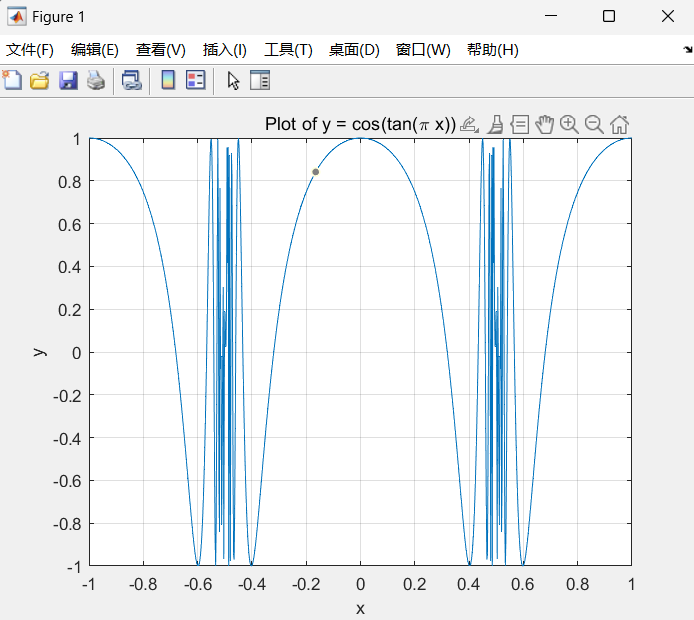
\includegraphics[width=0.75\linewidth]{3.2.png}


\end{figure}

\begin{figure}
    \centering
    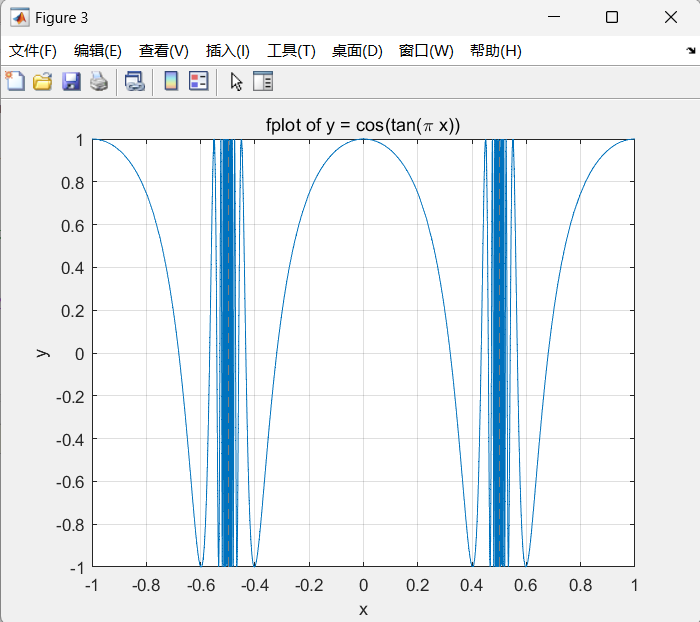
\includegraphics[width=0.75\linewidth]{3.11.png}
    
    
\end{figure}


\clearpage


\begin{figure}
    \centering
    
\includegraphics[width=1\linewidth]{++4.png}
    
    
\end{figure}

\par \textbf{思路简介}
\par 定义了参数方程,其中 x 和y 用参数t 表示,创建了t 的取值范围,并对这些值进行了求解,最后绘制出参数曲线。
\par \textbf{解答}

\begin{lstlisting}[
frame=single,
numbers=left,
style=Matlab-Pyglike]

x = @(t) t - (sin(t)).^3;
y = @(t) 1 - (cos(t)).^3;

t = linspace(0, 2*pi, 1000);

X = x(t);
Y = y(t);

figure;
plot(X, Y);
title('Plot of x = t - (sin(t))^3, y = 1 - (cos(t))^3');
xlabel('x');
ylabel('y');
grid on;

\end{lstlisting}

\par \textbf{实验结果}
\begin{figure}
    \centering
    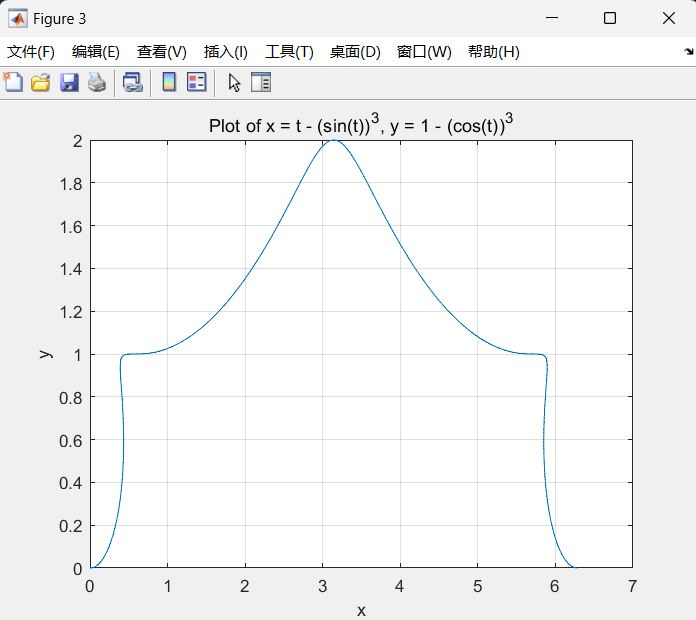
\includegraphics[width=0.75\linewidth]{4.1.png}
    
    
\end{figure}
\clearpage


\begin{figure}
    \centering
    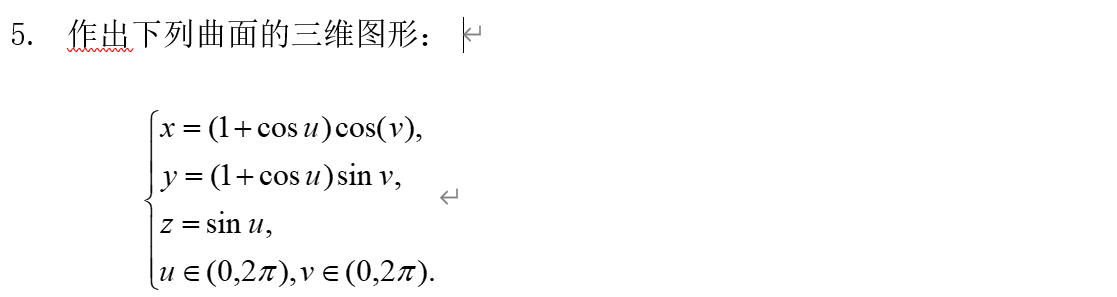
\includegraphics[width=1\linewidth]{++5.png}
    
    
\end{figure}

\par \textbf{思路简介}
\par meshgrid绘制由函数 x(u,v)、y(u,v) 和 z(u) 定义的参数曲面。
\par \textbf{解答}

\begin{lstlisting}[
frame=single,
numbers=left,
style=Matlab-Pyglike]
x = @(u,v) cos(v).*(1+cos(u));
y = @(u,v) sin(v).*(1+cos(u));
z = @(u)sin(u);
u = linspace(0, 2*pi, 1000);
v = linspace(0, 2*pi, 1000);
[X, Y] = meshgrid(u, v); 
Z = z(u);

figure;
plot3(x(X,Y), y(X,Y), Z);
title('3d Plot');
xlabel('x');
ylabel('y');
zlabel('z');
grid on;

\end{lstlisting}
\par \textbf{实验结果}
\begin{figure}
    \centering
    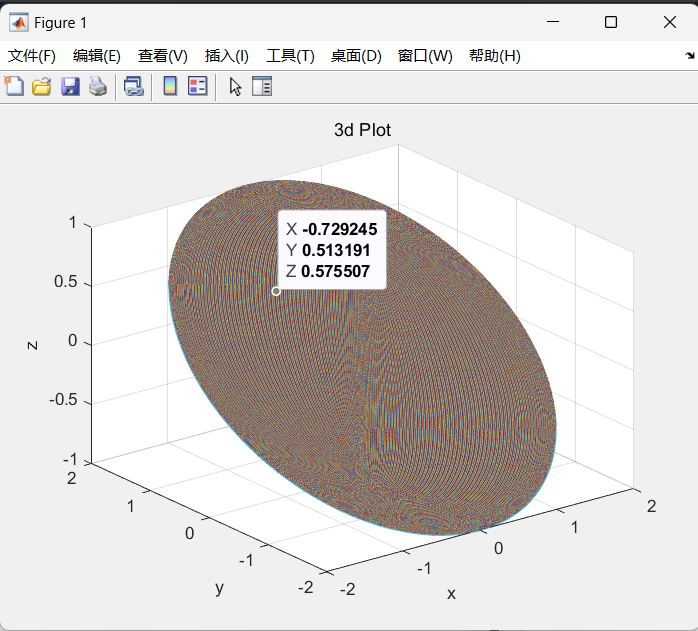
\includegraphics[width=0.75\linewidth]{5.1.png}
    
    
\end{figure}

\clearpage




\begin{figure}
    \centering
    
\includegraphics[width=1\linewidth]{++6.png}
    
    
\end{figure}
\par \textbf{思路简介}
\par 定义了一个名为 shuixian 的函数,用于找出在 100 到 999 之间的所有 "水仙花数"(Shuixianhua numbers),以及一个辅助函数 is\_shuixian,用于检查给定的数字是否是水仙花数。
\par \textbf{解答}

\begin{lstlisting}[
frame=single,
numbers=left,
style=Matlab-Pyglike]
function shuixian()
    disp('水仙花数:');
    for num = 100:999
        if is_shuixian(num)
            disp(num);
        end
    end
end

function result = is_shuixian(num)
    digit1 = floor(num / 100);
    digit2 = floor(mod(num, 100) / 10);
    digit3 = mod(num, 10);
    
    sum_of_cubes = digit1^3 + digit2^3 + digit3^3;
    
    result = sum_of_cubes == num;
end

\end{lstlisting}


\par \textbf{实验结果}

\begin{lstlisting}[
frame=single,
numbers=left,
style=Matlab-Pyglike]
>> hw6
水仙花数:
   153

   370

   371

   407
\end{lstlisting}
\clearpage





\begin{figure}
    \centering
    
\includegraphics[width=1\linewidth]{++7.png}
    
    
\end{figure}
\par \textbf{思路简介}
\par 首先定义了一个函数 shu(),然后在函数体内使用 for 循环遍历从 1 到 999 的数值。在每次循环中,使用 factorial() 函数计算当前数值的阶乘,然后与 200000 进行比较。
\par \textbf{解答}

\begin{lstlisting}[
frame=single,
numbers=left,
style=Matlab-Pyglike]
function shu()
    disp('最小的阶乘大于 200000的正整数:');
    for num = 1:999
        if factorial(num)>200000
            disp(num);
            break
        end
    end
end

\end{lstlisting}


\par \textbf{实验结果}
\begin{lstlisting}[
frame=single,
numbers=left,
style=Matlab-Pyglike]
>> hw7
最小的阶乘大于 200000的正整数:
     9
\end{lstlisting}

\clearpage




\begin{figure}
    \centering
    
\includegraphics[width=1\linewidth]{++8.png}
    
    
\end{figure}

\par \textbf{思路简介}
\par 调用名为gcd()和lcm()的函数来计算最大公约数和最小公倍数。
\par \textbf{解答}

\begin{lstlisting}[
frame=single,
numbers=left,
style=Matlab-Pyglike]

num1 = input('请输入第一个正整数:');
num2 = input('请输入第二个正整数:');


gcd_result = gcd(num1, num2);

lcm_result = lcm(num1, num2);

fprintf('输入的两个正整数 %d 和 %d 的最大公约数是:%d\n', num1, num2, gcd_result);
fprintf('输入的两个正整数 %d 和 %d 的最小公倍数是:%d\n', num1, num2, lcm_result);

\end{lstlisting}


\par \textbf{实验结果}
\begin{lstlisting}[
frame=single,
numbers=left,
style=Matlab-Pyglike]
>> hw8
请输入第一个正整数:15
请输入第二个正整数:963.
输入的两个正整数 15 和 963 的最大公约数是:3
输入的两个正整数 15 和 963 的最小公倍数是:4815
\end{lstlisting}

\clearpage

\begin{figure}
    \centering
    
\includegraphics[width=1\linewidth]{++9.png}
    
\end{figure}

\par \textbf{思路简介}
\par 使用 linspace 函数创建角度向量 theta,定义五角星的顶点。通过 cos 和 sin 函数计算五角星的x和y坐标。将五角星的x和y坐标分别存储到 x\_star 和 y\_star 数组中。创建一个新的图形窗口,并绘制初始五角星。使用 for 循环,以1度的增量逐步旋转五角星。将五角星的x和y坐标与旋转矩阵相乘来实现旋转。使用 drawnow 函数立即绘制更新后的图形。使用 pause 函数在每次迭代之间添加0.1秒的延迟,以控制动画的速度。
\par \textbf{解答}

\begin{lstlisting}[
frame=single,
numbers=left,
style=Matlab-Pyglike]

theta = linspace(0, 2*pi, 6);
x = cos(theta + pi/2); 
y = sin(theta + pi/2); 

x_star = [x(1:2:end) x(2:2:end)];
y_star = [y(1:2:end) y(2:2:end)];

figure;
starr = plot(x_star, y_star);
axis equal;
axis([-1.5 1.5 -1.5 1.5]);
title('Rotating Pentagram Animation');

angle = 0;

for i = 1:360
    x_rotated = x_star * cosd(angle) - y_star * sind(angle);
    y_rotated = x_star * sind(angle) + y_star * cosd(angle);
    
    set(starr, 'XData', x_rotated, 'YData', y_rotated);
    drawnow;
    
    pause(0.1);
    
    angle = angle + 1;
end

\end{lstlisting}


\par \textbf{实验结果}

\begin{figure}[h]
 
\begin{minipage}{0.32\linewidth}
 
\vspace{3pt}
 
\centerline{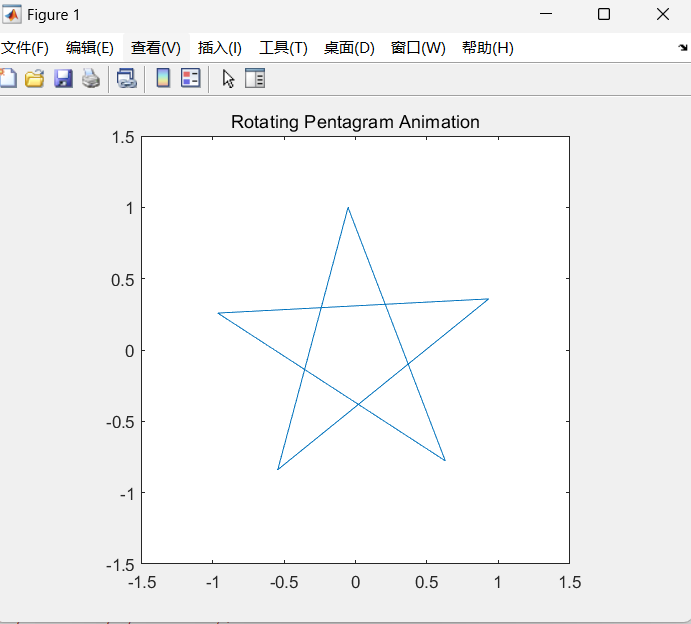
\includegraphics[width=\textwidth]{9.1.png}}
 
 
\centerline{Image1}
 
\end{minipage}
 
\begin{minipage}{0.32\linewidth}
 
\vspace{3pt}
 
\centerline{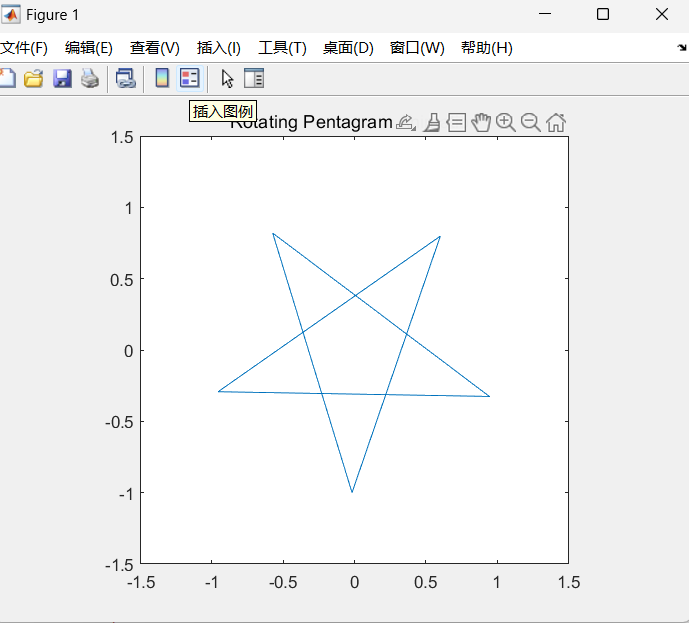
\includegraphics[width=\textwidth]{9.2.png}}
 
 
 
\centerline{Image2}
 
\end{minipage}
 
\begin{minipage}{0.32\linewidth}
 
\vspace{3pt}
 
\centerline{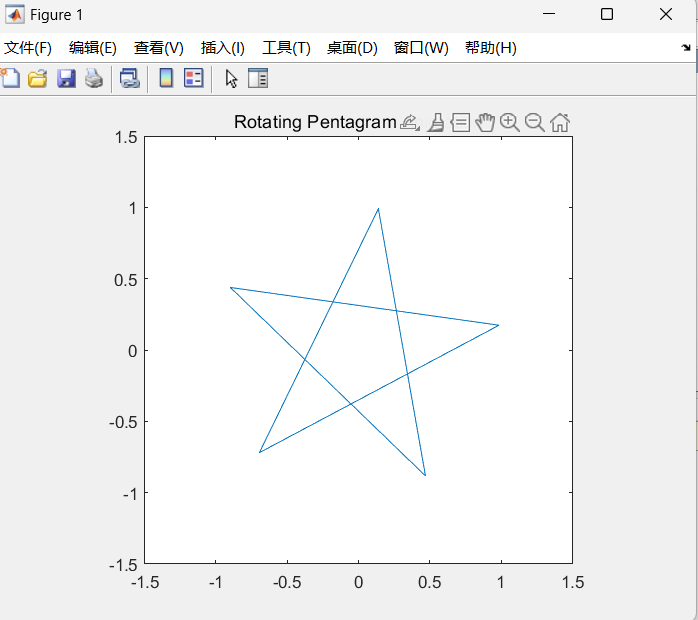
\includegraphics[width=\textwidth]{9.3.png}}
 
 
 
\centerline{Image3}
 
\end{minipage}
 
 
 
\caption{五角星动画截图 }
 
\label{fig4}
 
\end{figure}


\clearpage




\begin{figure}
    \centering
    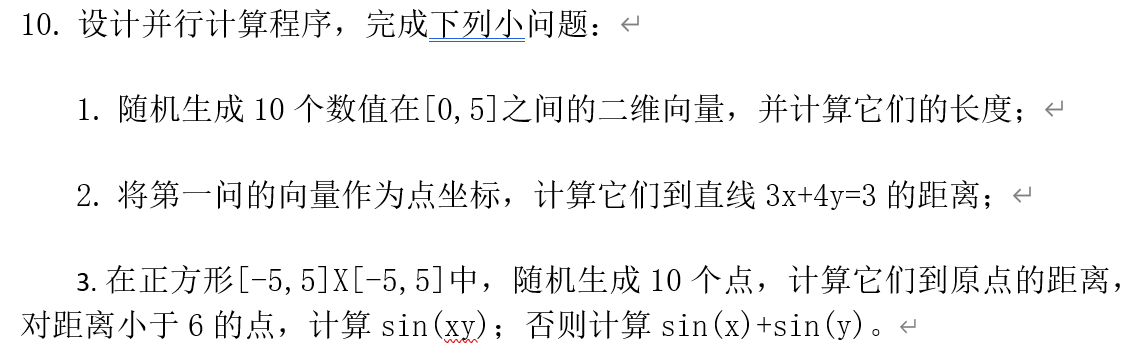
\includegraphics[width=1\linewidth]{++10.png}
    
    
\end{figure}


\par \textbf{思路简介}
\par rand生成了一些随机的二维向量和点,然后计算了它们的长度或到直线的距离,并根据条件计算了对应的值。
\par \textbf{解答}

\begin{lstlisting}[
frame=single,
numbers=left,
style=Matlab-Pyglike]

num_vectors = 10;
vectors = rand(num_vectors, 2) * 5;

lengths = sqrt(vectors(:,1).^2 + vectors(:,2).^2);

disp('随机生成的二维向量及其长度:');
disp([vectors lengths]);
a = 3;
b = 4;
c = -3;

distances = abs(a*vectors(:,1) + b*vectors(:,2) + c) ./ sqrt(a^2 + b^2);

disp('向量到直线的距离:');
disp(distances);


num_points = 10;
points = rand(num_points, 2) * 10 - 5; 

distances = sqrt(points(:,1).^2 + points(:,2).^2);

values = zeros(num_points, 1); 
for i = 1:num_points
    if distances(i) < 6
        values(i) = sin(points(i,1) * points(i,2));
    else
        values(i) = sin(points(i,1)) + sin(points(i,2));
    end
end

disp('点到原点的距离及相应的值:');
disp([distances values]);

\end{lstlisting}


\par \textbf{实验结果}


\begin{lstlisting}[
frame=single,
numbers=left,
style=Matlab-Pyglike]
>> hw10
随机生成的二维向量及其长度:
    1.7583    0.3793    1.7987
    4.1541    0.2698    4.1629
    2.9263    2.6540    3.9506
    2.7486    3.8958    4.7679
    4.5860    4.6701    6.5453
    1.4292    0.6495    1.5699
    3.7860    2.8441    4.7353
    3.7686    2.3470    4.4397
    1.9022    0.0595    1.9032
    2.8391    1.6856    3.3018

向量到直线的距离:
    0.7584
    2.1083
    3.2790
    4.1658
    5.8876
    0.7771
    3.9469
    3.5387
    0.5889
    2.4520

点到原点的距离及相应的值:
    3.4142    0.9950
    5.0971    0.3135
    3.3029   -0.9194
    4.1432    0.9244
    4.8232   -0.8097
    3.4140   -0.1802
    2.4011   -0.7888
    5.1951    0.9781
    4.6232   -0.9919
    2.5469   -0.9890
\end{lstlisting}
\clearpage

\end{document}